\section{Evaluation}

This section evaluates the result of different clusterings with different weights of the used features.
Multiple clusterings with different feature weight were processed to get a deeper understanding
of the correlation between the features and the demand development.

{\small
\begin{table}[ht]
  \caption{Different feature weights and their result}
  \label{table:clusteringComparison}
  \begin{tabular}{cccccccc}
    Nr. &  Clusters & Avg Rating & Level & High Avg & Big Cluster & Weight {\tiny Size Industry Location & Tree depth} \\ \hline
    1&          8      & 1.0500     & 45    & 34\%     & 732 \(911\) &  0,0,1          & 777 \\
    2&          4      & 1.0560     & 119   & 22\%     & 233 \(357\) &  0,1,0          & 352 \\
    3&          3      & 1.0356     & 148   & 27\%     & 136 \(211\) &  1,0,0          & 284 \\
    4&          4      & 0.7597     & 61    & 27\%     & 46 \(64\)   &  1,1,1          & 107 \\
              %8      & 0.7375     & 51    & 45\%     & 10 \(42\)   & 2,4,1           & 61 \\
    5&          7      & 0.8480     & 51    & 7\%      & 43 \(94\)   & 2,2,1           & 94 \\
    6&          6      & 0.8556     & 60    & 7\%      & 43 \(99\)   & 2,8,1           & 103 \\
  \end{tabular}
\end{table}

}

\subsection{Correlation of company closeness and need development}

Table \ref{table:clusteringComparison} shows the resulting measurements regarding to the different feature weights.
To see what impact each feature has without the influence of the other ones, an own cluster combination for each
feature was created \footnote{See tablerows 1-3 in \ref{table:bestClustering}}.

The results for this combination were quite similar. Their average rating is between 1.03 and 1.05 whereas
the tree depth differs a lot. A hierarchical clustering always produces a tree as its outcome structure. This
tree represents the clustering. Each node within this tree represents an own cluster that contains every child element
of this node. So the deeper the tree the more one company clusters \footnote{A one company cluster is a cluster with only one element}
it contains. One company clusters are bad for deducing a correlation of company closeness and need development because
a company within a one company cluster can not have influence on any other companies within this cluster.
According to the results for clusterings with single weights only, the clustering resulted from the location weighted
tree has a much higher depth than any other result set. Therefore the location itself as a result is useless.
The other two single weighted trees are useless for predictions as well. Their clusters show a balanced demand
development for each of the products. So they are not suited for demand predictions by themselves.

This result is not astonishing as economic processes are very complex and can not be described by a single
measurement. Thats why we had a look at the influence of all three of the features. According to
Porter \cite{CompanyClusters} and Webster and Wind \cite{BusinessBuyingBehavior} industry and location
do both have a high influence. So we had a look at combination where this features where wheighted more than
the size feature.

The unexpected result was that the evenly ditributed weight to all of the three features leads the best outcome.
It has a similar depth like table rows number 5 and 6 but much better average rating which is the most interesting
measurement to look for. Even if it only covers two thirds of the other two result sets it has a higher prediction potential.

\begin{figure}[ht]
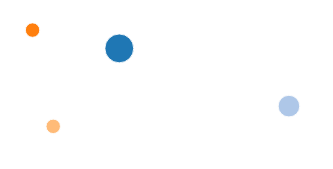
\includegraphics[scale=1]{bestClustering.png}
\centering
\caption{Visualized cluster for the cluster combination with the best rating}
\label{fig:bestClustering}
\end{figure}

Figure \ref{fig:bestClustering} shows the 4 clusters belonging to table row number 4 and the distance between each
of the cluster. The one company clusters are ignored in this visualization because they do not provide any
further value. Even if this cluster combination provides the best average rating it is still not good engough
to perform any useful predictions. On the one hand it covers only around a twentieth of the overall companie set
and on the other hand the cluster score of 0.75 is still to high for reliable demand forecasts.

% why or why not may companies raise certain needs ~
\subsection{How could the result could be improved?}











To test what influence each feature has
we will have a look at the

 Therefore the first approach weights the location and industry 0.45 each and the size 0.1 times.

Show coverage of companies within cluster that match a product related demand. At the beginning , midtime and at the end.
Evaluate the goodness of the feature distribution by this development.

Showing that the clustering makes sense. Explain why its ok to ignore clusters that are only a company by itself. ->
To show the spreading over time within a cluster to show the well choseness of a cluster cant be shown with one company
cluster
